\chapter{Empirical Validations}\label{chap:empirical_validations}
In this chapter, we evaluate the predictions of the model developed in \cref{chap:a_unifying_model} against high precision eye-tracking data from \textcite{naher_primate_saccades}, described in \cref{sec:model_setup}. Motivated by established spatiotemporal signatures of gaze during visual search, we examine three key dynamical features: (1) theta-rhythmic saccades, (2) gamma-scale \qtyrange{40}{100}{\hertz} fixational ocular drift, and (3) global superdiffusion across spatial scales \cite{mahanama_eye_2022, martinez-conde_role_2004}. Our unifying framework seeks to explain these phenomena through network-level neural activity, including the proposed connection between microtremor and neural gamma, theta-gamma coupling, and the monoscaling of superdiffusion across spatial scales.

\Cref{sec:theta_rhythmicity_of_saccades} examines theta rhythmicity of saccades, comparing the model's transitional rhythmicity with the saccade timing in the data. \cref{sec:gamma_oscillations} examines gamma-scale oscillations during visual fixations, testing the model's local high-frequency harmonic oscillations against fixational drift. \cref{sec:search_superdiffusion} examines superdiffusion in search, assessing whether the global spatial statistics of gaze are consistent with Lévy superdiffusion. Finally, \cref{sec:spatiotemporal_predictions} presents the spatiotemporal predictions of the model across these scales and discusses how they unify the experimental and modelling findings above.

%%% 3.1 Theta rhythmicity of saccades
\section{Theta rhythmicity of saccades}\label{sec:theta_rhythmicity_of_saccades}
The approximate \qty{200}{\ms} timescale of human saccades has long existed experimentally \cite{meyer_rhythmicity_1966, saccadic_rhythm_1986, chota_rhythmic_2018, shaverdi_orchestration_2023}. A direct measure of saccade rhythmicity is the direct measurement of the spread of the ISI distribution, assuming a large lognormal spread of intervals $\Delta t$. This can be used to construct a measure called the Rhythmicity Index (RI):
\begin{equation}
	\text{RI} = \frac{1}{\text{CV}_{\ln}}, \qquad \text{CV}_{\ln} = \sqrt{e^{\sigma_{\ln}^2} - 1}
\end{equation}
where $\sigma_{\ln}$ is the standard deviation of the distribution of ISIs in log-space $\ln \Delta t$, with $\text{CV}_{\ln}$ often called the geometric CV. This $\text{RI}$ is an effective measure of the spread of a strictly positive distribution. A Poisson distributed variable will give $\text{RI}=1$, whereas it is found that for the ISI distribution of subjects considered here for a random NOISE condition is $\text{RI} = 2.69$ \cite{naher_primate_saccades}.

\subsection{Local rhythmicity of saccades}
The recent discovery of the strength of saccade rhythmicity by \textcite{naher_primate_saccades} and others \cite{zubair_eye_2026} required a deep understanding of the rhythmicity of biological systems. A challenge that is often present in biological systems is that timescales are not driven by a perfect clock, but instead the characteristic timescales of certain regular patterns in the brain. As such, the \qty{200}{\milli \second} estimate for saccades during a visual search is not expected to be a universal timescale across subjects and trials. Instead, the model used for such processes in neuroscientific works is a noisy rise-to-threshold model, where a random walk is constructed, and when it reaches a goal, a decision is made \cite{naher_primate_saccades} [CITE]. The noise-driven rise for this process is expected to have a rate which is slowly varying about a characteristic timescale, in the case of saccades around \qtyrange{2}{6}{\hertz}. Since this slowly varying rate is expected to be stable for a single individual and a single trial, we consider a local measure of rhythmicity for the intervals between the saccades within a timseries, called the Inter-Saccadic-Intervals (ISI). Such a metric can be proposed---as developed by \cite{naher_primate_saccades}---with the local Rate-Corrected Rhythmicity Index (RCRI):
\begin{equation}\label{eq:RCRI}
	\text{RCRI} = \frac{1}{1 + \langle \text{CV}_2 \rangle}, \qquad \text{CV}_2(i) = 2\frac{\|\Delta t_{i+1} - \Delta t_{i} \|}{\Delta t_{i+1} + \Delta t_{i}}
\end{equation}
which allows quantification of purely local rhythmicity, comparing each interval $\Delta t_{i+1}$ to it's predecessor $\Delta t_{i}$, and averaging across all intervals considered $i$, usually a single subject. The results of such an analysis have resulted in two key conclusions. Firstly, human saccades are very strongly rhythmic, with $\text{RCRI}\approx0.76$ for the subjects as described in \cref{sec:model_setup} depending on condition. Secondly, it has been found that the instantaneous saccade rate is a strong predictor for the local saccade rhythmicity $\text{RCRI}$, with a correlation calculated at $\rho=0.39, P=0.001$, with saccade rate found to be a significant predictor of $\text{RCRI}$ with $\beta=\qty{0.0114}{\hertz^{-1}}, P=0.014$

those particular individuals and trials binned with a higher saccade rate correlate with higher RCRI and thus stronger comparable rhythmicity \cite{naher_primate_saccades}, as shown in \cref{fig:rate-RCRI}.
\begin{figure}[htbp]
	\centering
	\begin{subfigure}[T]{0.45\textwidth}
		\centering
		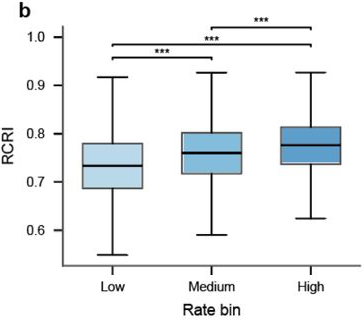
\includegraphics[width=\linewidth]{figures/RCRI.png}
		\caption{\textbf{Rate-corrected rhythmicity index (RCRI) is positively correlated with saccade rate.} Collaborators \textcite{naher_primate_saccades} uncovered this statistically significant result, which implies that shorter inter-saccadic intervals (ISIs) will result in more regular ISIs, which corresponds to stronger kernel dynamics as defined in \cref{subsec:adaptive_kernel_dynamics}.}
		\label{fig:rate-RCRI}
	\end{subfigure}
	\hfill
	\begin{subfigure}[T]{0.45\textwidth}
		\centering
		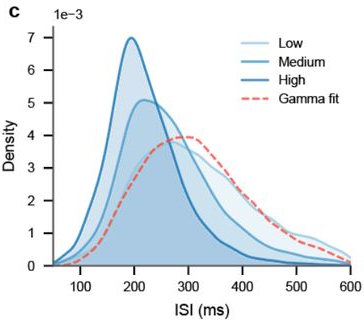
\includegraphics[width=\linewidth]{figures/ISI.png}
		\caption{\textbf{The probability distribution of inter-saccadic intervals (ISIs) are tightly distributed in a Gamma-10 distribution.} Our collaborators in \textcite{naher_primate_saccades} find that saccades are more locally rhythmic than previously considered. In particular, the ISI distribution is a tight Gamma-10 distribution, but the ISI timeseries is strongly locally rhythmic, as captured by the rate-corrected rhythmicity index (RCRI).}
		\label{fig:gamma_fits}
	\end{subfigure}
	\caption{}
	\label{fig:local_rhythmicity}
\end{figure}
\subsubsection*{Interpretations of local rhythmicity and saccade rate for a model of gaze dynamics}
These results support our unified stochastic-informative formulation of gaze dynamics. We have shown good agreement between the tight distribution of modelled ISIs, more closely locally. We have also introduced a natural parameter $\tau$ with which to modulate the slowly varying theta-scale saccade rate. This also connects the dynamics of information gathering with the dynamics of regular attention in a search task. The results that rhythmicity is strongest where a task contains nearly identical searched objects is encouraging for this information-driven saccade rate theory. A correlation between high saccade rate and high rhythmicity is predicted from the origin of regular dynamical-informational transitions as described in \cref{sec:dynamical-information_adaptation}, where a stronger kernel produces more rhythmic transitions, and a weaker kernel will approach an arrhythmic Poisson point distribution of ISIs, reducing the RCRI, as predicted.

%%% 3.2 Gamma oscillations in visual fixations
\section{Gamma oscillations during visual fixation}\label{sec:gamma_oscillations}


\subsection{Previous treatment as \textit{ocular microtremor}}

\subsection{Analysis of fixational Fourier spectra}

% \begin{figure}[htbp]
%     \centering
%     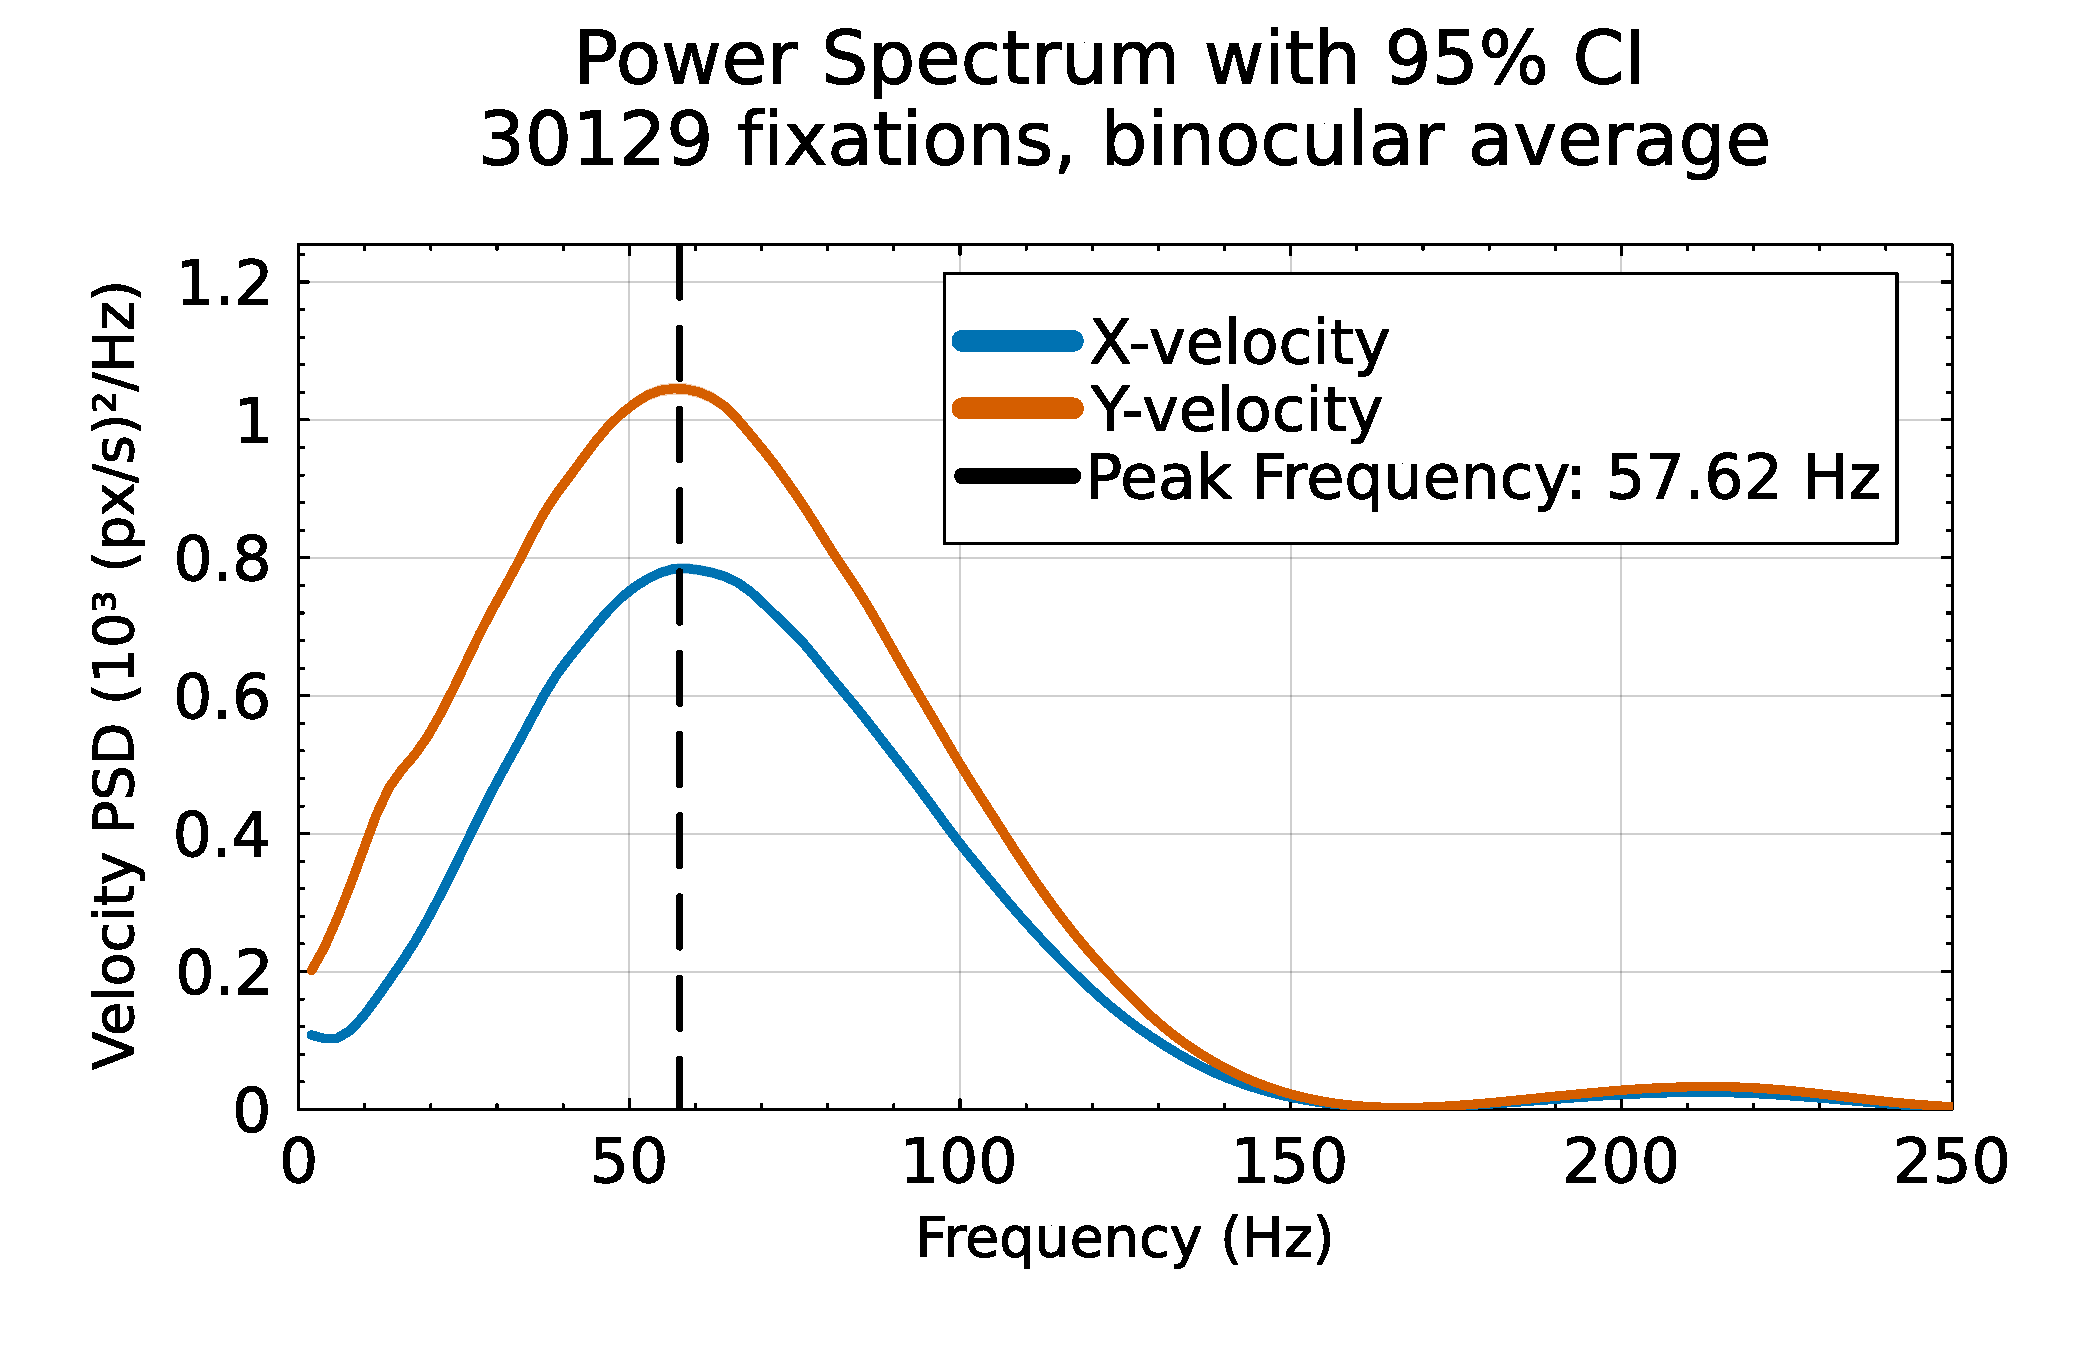
\includegraphics[width=\linewidth]{figures/fixation_psd_plot.pdf}
%     \caption{Caption.}
%     \label{fig:main}
% \end{figure}


% \begin{figure}[htbp]
%     \centering
%     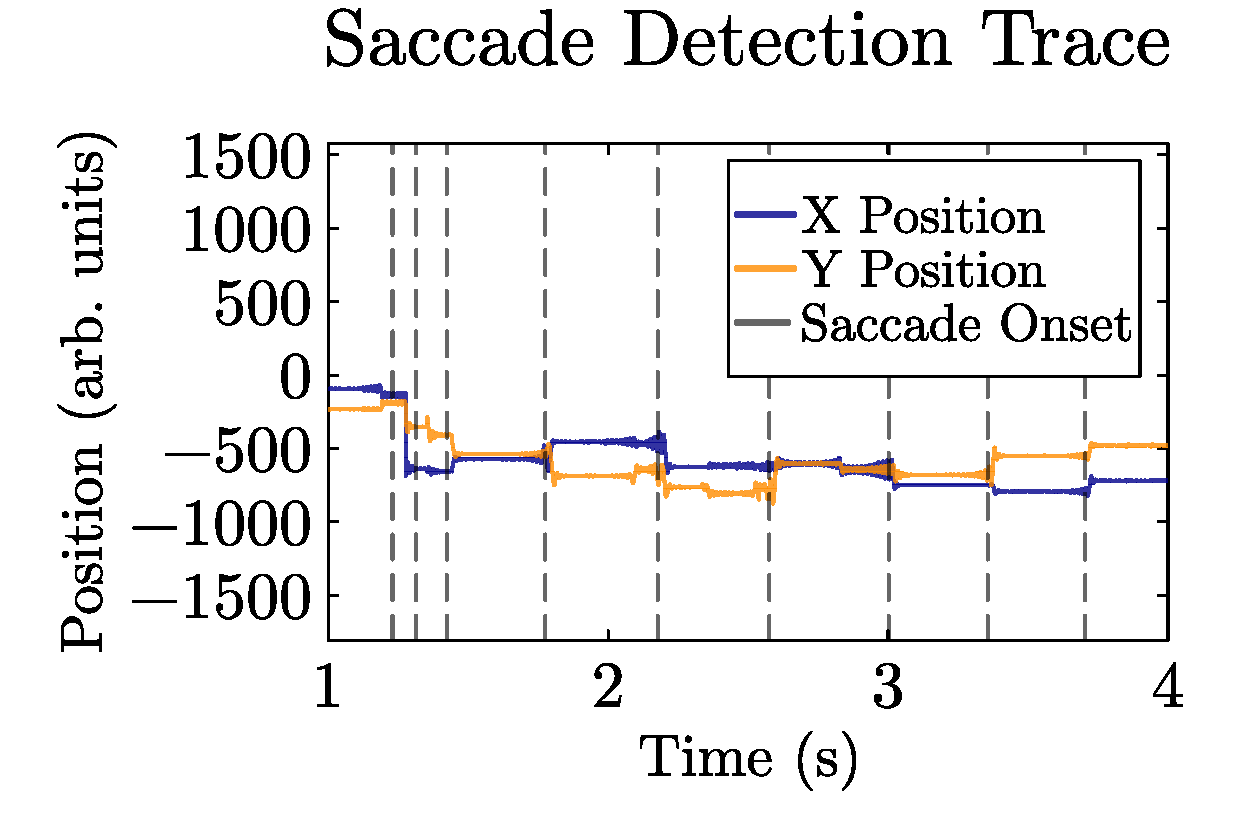
\includegraphics[width=\linewidth]{figures/saccade_trace.pdf}
%     \caption{Caption.}
%     \label{fig:main}
% \end{figure}

%%% 3.3 Search superdiffusion
\section{Search superdiffusion}\label{sec:search_superdiffusion}
Superdiffusion is often a prominent pattern in natural dynamical systems, and its presence points to a self-similar fractal structure. Such dynamics have not been the focus of other studies, and visual trajectories have often been treated as fixational Brownian motion, externally interrupted by saccades, which would suggest separate regimes of diffusion across $q$. We present here a monoscaling superdiffusive pattern in gaze dynamics across a wide range of scales. Many studies that have described eye movement dynamics as normally diffusive stem from the sensitivity of data-processing choices in detecting anomalous diffusion at confined boundaries, such as fixations. Conventional analyses often inadvertently obscure critical spatiotemporal features.

The most important methodological choice in accurately characterising visual diffusion patterns is to time-average displacements. As demonstrated by \textcite{vilk_strong_2025}, aggregating data across disparate temporal regimes can wash out localised scaling behaviours, yielding normal diffusion as an artefact. Studies that construct regimes of normality and subdiffusive regimes are thus common in the study of eye movements, but this ignores continuous-time superdiffusion, which we unify across multiple scales. For such studies, see \cite{lencastre_dynamical_2025, leroux_random_2021, roberts_fixational_2013, collewijn_significance_2008}.

\subsubsection*{Analysis of multiscale superdiffusion in eye-tracking data}
We analyse the binocular-averaged gaze trajectories over all 22 human subjects provided from the study in \textcite{naher_primate_saccades}, as described in \cref{sec:model_setup}. From the onset of the search task, we time-average the fractional absolute displacements $\langle \|\Delta \textbf{x}(\Delta t) \|^q \rangle $ for 30 values of $q$ linearly separated from $q=0.1$ to $q=3.0$. These fractional absolute moments are evaluated over all valid time lags $\Delta t < \qty{1000}{\ms}$ with a resolution of $\Delta t = \qty{1}{\ms}$. All intervals containing NaN values (such as blinks) are discarded. We then ensemble-average these displacements across all subjects. These results are shown in \cref{fig:search_superdiffusion}\textbf{a-d)}.

We perform a linear best-fit of the gaze and model fractional moments in log-log space $M_q(\Delta t)$ as defined in \cref{eq:Mq} to find short-time power-law diffusive scaling with time, thus sampling from our moment spectrum function $\lambda(q)$ as defined in \cref{eq:MFD}. Each of these fractional moments is overlaid in \cref{fig:search_superdiffusion}\textbf{a,c)}, and their slopes are plotted in \cref{fig:search_superdiffusion}\textbf{b,d)}. The moment spectrum function $\lambda(q)$ is thus found to have a good fit to $\lambda(q) = (0.897 \pm 0.007)q$ with an error in the fit of $R^2 = 0.999$. This behaviour yields monoscaling across spatial scales, from fixations to saccades. The corresponding Lévy exponent given such linear monoscaling in $\lambda(q)$ is thus found to be $\alpha = 1.115 \pm 0.007$.
\subsection{Spectrum of fractional moments}\label{subsec:spectrum_of_fractional_moments}
\Cref{fig:search_superdiffusion} summarises the scaling of the time-averaged fractional absolute displacements. For comparison of the various scaling exponents, we define a rescaled moment function $M_q(\Delta t)$ to give a good comparison of the spectrum of moments under the same dimensions of distance. $M_q(\Delta t)$ is here defined
\begin{equation} \label{eq:Mq}
    M_q(\Delta t) = C_q \langle \|\Delta\mathbf{x}(\Delta t)\|^{q} \rangle^{1/q} \sim \Delta t^{\lambda(q) / q}
\end{equation}
with $C_q$ defined such that $M_q(\Delta t_{\text{min}})=1$ to give a shared origin at the first time lag $\Delta t$. Small $q$ gives strong weight to the small, frequent displacements of fixational motion, while large $q$ weights the rare, large displacements which are given in saccades. The shape of $\lambda(q)$, therefore, examines the spectrum of exponents that may describe superdiffusion at any scale. A linear spectrum, $\lambda(q) = q/\alpha$, is monoscaling: all moments grow with the same exponent, as for a self-similar Lévy process with stability index $\alpha$. A nonlinear spectrum is the general case found in many systems called strong anomalous diffusion, which consists of two dynamical strategies stitched together at different scales \cite{vilk_strong_2025, cagnetta_strong_2015, castiglione_strong_1999, wang_strong_2020}. See \cref{subsec:levy_motion} for a further discussion of mono- and multiscaling, and \cref{fig:SANDvsmono} for its schematic representation.

\Cref{fig:search_superdiffusion} shows the rescaled moments $M_q(\Delta t)$ for the human eye-tracking data and modelled gaze. The slope of each curve in log--log space is robustly linear, with constant slope $\lambda(q)/q$. Lévy monoscaling predicts a slope across the entire spectrum, with $\lambda(q) = q/\alpha$. For comparison, Brownian motion ($\alpha = 2$) has slope $1/2$ and ballistic motion has slope $1$ across the entire spectrum $q$. The monoscaling exponent is found by performing a linear regression on our spectrum $\lambda(q)$. \Cref{fig:search_superdiffusion}\textbf{b,d)} shows these fitted exponents $\lambda(q)$ against $q$. The linear fit is good, with $\lambda(q) = (0.897 \pm 0.005)\,q$ and $R^2 = 0.999$, across the whole considered range $0.1 \le q \le 3.0$. This gives a Lévy index $\alpha = 1.115 \pm 0.007$, which is well below the Brownian value of $2$ and so indicates strong superdiffusion. Because a linear regression well describes the spectrum, there is no crossover in scaling between the low-$q$ moments that probe fixational motion and the high-$q$ moments that probe saccades. A single exponent describes both, validating our unifying model across both scales of study in gaze dynamics, derived naturally from FNS dynamics.
\begin{figure}[htbp!]
	\centering
	\begin{subfigure}[t]{0.49\textwidth}
		\centering
		\panel{a)}{figures/superdiffusion/data/rescaled_moment_spectrum_data.pdf}
		\label{subfig:fad_data}
	\end{subfigure}
	\hfill
	\begin{subfigure}[t]{0.49\textwidth}
		\centering
		\panel{b)}{figures/superdiffusion/data/lambda_vs_q_fit_data.pdf}
		\label{subfig:scaling_order_data}
	\end{subfigure}
	\vfill
	\begin{subfigure}[t]{0.49\textwidth}
		\centering
		\panel{c)}{figures/superdiffusion/model/rescaled_moment_spectrum.pdf}
		\label{subfig:fad_model}
	\end{subfigure}
	\hfill
	\begin{subfigure}[t]{0.49\textwidth}
		\centering
		\panel{d)}{figures/superdiffusion/model/lambda_vs_q_fit.pdf}
		\label{subfig:scaling_order_model}
	\end{subfigure}
    \caption{\textbf{The model reproduces the monoscaling superdiffusion of human visual search through a linear spectrum of moments.} Rescaled moments $M_q(\Delta t)$ (\cref{eq:Mq}) and fitted scaling exponents $\lambda(q)$ for 30 values of $q$ spaced linearly from $0.1$ to $3.0$. \textbf{Top row:} binocular-averaged gaze data from the 22 subjects of \textcite{naher_primate_saccades} (1846 trajectories, mean duration \qty{5}{\s}). \textbf{Bottom row:} 500 trajectories simulated from the model of \cref{chap:a_unifying_model} (mean duration \qty{15}{\s}). \textbf{(a,c)}~Moments on log--log axes. The shaded region denotes the fitting regime, and the dashed line shows the $q=2$ fit, which recovers the square-root scaling of the traditional MSD. Ringing oscillations in the low--$q$ moments result from the highly regular harmonic oscillations that model gamma-scale OMT. \textbf{(b,d)}~The spectra are linear, $\lambda(q) = q/\alpha$, in both cases: $\alpha = 1.115 \pm 0.007$ for the data ($R^2 = 0.999$) and $\alpha = 1.091 \pm 0.005$ for the model, showing robust superdiffusion across scales, compared with $\alpha = 2$ recovering Brownian motion.}
    \label{fig:search_superdiffusion}
\end{figure}
\subsubsection*{Implications of monoscaling superdiffusion}
The most important implication of this particular superdiffusion result is that the strong monoscaling of visual search trajectories with Lévy index $\alpha = 1.115$ is robustly multiscale. The robust linear scaling of $\lambda(q)=\frac{q}{\alpha}=\frac{q}{1.115}$ across a spectrum of $q$-values $0 < q < 3$ is important, as it suggests an identical process driving both fixational eye movements --- including tremor, drifts, and microsaccades --- with small relative values of $\| \Delta \textbf{x}\|$ emphasised with low values of $q$, as well as large nonlocal saccades with large relative values of $\| \Delta \textbf{x} \|$, emphasised through large values of $q$. Importantly, this validates our construction of a continuous-time unified model of eye movements, unified across all spatiotemporal scales of visual search.


%%% 3.4 Spatiotemporal predicions
\section{Spatiotemporal predictions from the model}\label{sec:spatiotemporal_predictions}

Throughout this chapter, we present a novel physics-inspired analysis of a standard gaze-tracking experiment during visual search which yields new results and predictions of gaze dynamics. In particular, the approximate timescale of saccades has been known since the beginning of the field of eye movement research, whereas the significance of the rate-corrected local rhythmicity is a very recent result only discovered in the year of this present work. OMT as a phenomenon has been found in the literature \cite{graham_ocular_2023}, however no consensus exists as to it's importance in the functioning of gaze, and it has never been linked to a computational role of gamma-scale rhythms. Lastly, the mathematical analysis of search superdiffusion of gaze has only been recently undertaken in the literature, and without the well-motivated link to a model of gaze we present here. However, another benefit of comparing the generative unifying model presented in \cref{chap:a_unifying_model} to the data is that further dynamical predictions outside of the present literature can be made. Thus, we present experimental paradigms and features of this model which are being developed to better understand visual searching.
\subsection{Saliency-frequency coupling in contrast-dependant search tasks}
OMT frequency is here hypothesised to be the result of a harmonic oscillations in the control of the path of the eye during fixation tasks. An experiment may be designed in which targets with various degrees of contrast are presented to be searched. High contrast, localised points, such as tight, high spatial frequency Gabor patches, would produce localised saliency wells with low $\sigma_{\text{fix}}$. Whereas, low contrast, large low spatial frequency patches would produce saliency wells with a large width $\sigma_{\text{fix}}$. High contrast wells would correspond to shorter theta timescales, quadratic in the effective saliency well size as in \cref{eq:theta_rhythm}, and a microtremor rhythm which is approximately inverse to the effective saliency well size as in \cref{eq:resonant_frequency}. The effect of visual contrast has been found to be significant in gamma frequency in the visual system, and this quantitative relationship provides an experimental prediction of the relationship between three data points: $t_{\theta}, f_{\text{peak}},$ and $k_{\text{Gabor}}$. A simple regression analysis can be achieved here to find correlations between spatial frequency $k_{\text{Gabor}}$ and the visual theta-rhythm $t_{\theta}$ and the $f_{\text{peak}}$. It can then also be tested if these effects are consistent with a potential well of variable size, such that $t_{\theta} \propto \sigma_{\text{fix}}^{-2}$ and $f \propto \sigma_{\text{fix}}^{-1}$
\subsection{Smooth pursuit predictions and parametric-fitting techniques}
Another experimental paradigm which provides insight into the behaviour of the control of visual trajectories. In particular, the exact same model can be examined in the behavioural paradigm of smooth tracking of a moving object. In particular, a typical experiment would be the tracking of a smoothly moving pendulum. It is realistically found that a typical eye movement trace contains discontinuous micro-saccades during smooth pursuit, and discontinuous catch-up saccades. In particular, we expect from the model that the instability will be most present in the periods of stability when kernel deposition is strongest. Further experiments could also find the behaviour of dynamics in phase space $\alpha/\beta/\gamma/t_{\theta}$ for different neurological conditions. For instance, it is well-known that schizophrenia effects the 

%%% Summary
\section*{Summary}
After examining our proposed model in depth, we have now compared to real human gaze data. This work has provided a dynamical explanation of the recently discovered significant regularity of saccades during a search task as a coupling between model dynamics and information through kernel deposition. We then made the novel prediction of gamma-scale oscillations in fixation dynamics, which was validated under the present data analysis. This component of fixational dynamics has rarely been studied as a coherent aspect of neural dynamics; we are the first to provide a modelled explanation of its neural origin. Finally, we presented the prediction of our model of unified fluctuation-driven superdiffusive motion across all spatial scales. By analysing fractional $q$--moments, we found that gaze trajectories are characterised by a single superdiffusive exponent across all scales, unifying the dynamics of fixations and of saccades under a single model. Finally, we suggest further experimental methods to test further quantitative predictions of the model designed to examine attention in the brain through the study of gaze dynamics.